\documentclass[a4paper, 11pt]{article}

\usepackage[left=2cm, right=2cm, top=2cm, bottom=2cm]{geometry}

\usepackage[utf8]{inputenc} 
\usepackage[T1]{fontenc}      
\usepackage[french,english]{babel}  
\usepackage{lmodern}

\usepackage{amsmath, mathtools}
\usepackage{amssymb}
\usepackage{amsthm}
\usepackage{empheq}

\usepackage{graphicx}
\usepackage{subfig}

\usepackage{listings}
\usepackage{color} %red, green, blue, yellow, cyan, magenta, black, white
\definecolor{mygreen}{RGB}{28,172,0} % color values Red, Green, Blue
\definecolor{mylilas}{RGB}{170,55,241}

\usepackage{mathtools}
\DeclarePairedDelimiter\ceil{\lceil}{\rceil}

\lstset{language=Matlab,%
    %basicstyle=\color{red},
    breaklines=true,%
    morekeywords={matlab2tikz},
    keywordstyle=\color{blue},%
    morekeywords=[2]{1}, keywordstyle=[2]{\color{black}},
    identifierstyle=\color{black},%
    stringstyle=\color{mylilas},
    commentstyle=\color{mygreen},%
    showstringspaces=false,%without this there will be a symbol in the places where there is a space
    numbers=left,%
    numberstyle={\tiny \color{black}},% size of the numbers
    numbersep=9pt, % this defines how far the numbers are from the text
    emph=[1]{for,end,break},emphstyle=[1]\color{red}, %some words to emphasise
    %emph=[2]{word1,word2}, emphstyle=[2]{style},    
}

\begin{document}
\title{Rendu TP4 Imagerie sous-pixellique}
\author{Yoann Pradat}
\maketitle

\paragraph{Exercice 11}

\textbf{1.} La fonction \texttt{perdecomp} calcule la periodisée d'une image numérique $u \in \mathbf{R}^{\Omega}$ avec $\Omega =
\{0, \dots, M-1\}\times\{0, \dots, N-1\}$ par calcul de la transformée de Fourier discrète de $s$, inversion de cette
transformée de Fourier et ensuite soustraction $per(u) = u-s$. \\

En effet d'après le cours la transformée de Fourier de $s$ est donnée par

\begin{equation*}
  \forall q,r \in \Omega \backslash \{0,0\} \quad \hat{s}[q,r] = \frac{0.5\hat{v}[q,r]}{2-\cos(\frac{2\pi q}{M}) -
  \cos(\frac{2\pi r}{N})}
\end{equation*}

et $v = v_1 + v_2$ est définie par rapport aux valeurs de $u$ aux bords et aux coins. La variable \texttt{v} de taille
\texttt{ny$\times$nx} = $M\times N$ calcule dans la fonction \texttt{perdecomp} les valeurs de $v$. On définit ensuite matricielle les
quantités $\cos(\frac{2\pi q}{M})$ et $\cos(\frac{2\pi r}{N})$ puis on calcule la transformée de Fourier inverse du
quotient donné par l'équation ci-dessus c'est-à-dire de $\hat{s}$. Une fois que l'on connaît la composante \og smooth
\fg de l'image on en déduit sa périodisée par soustraction. \\

\textbf{2.} On applique la décomposition précédente à l'image “lena.pgm” par exemple

\begin{figure}[!h]
\centering
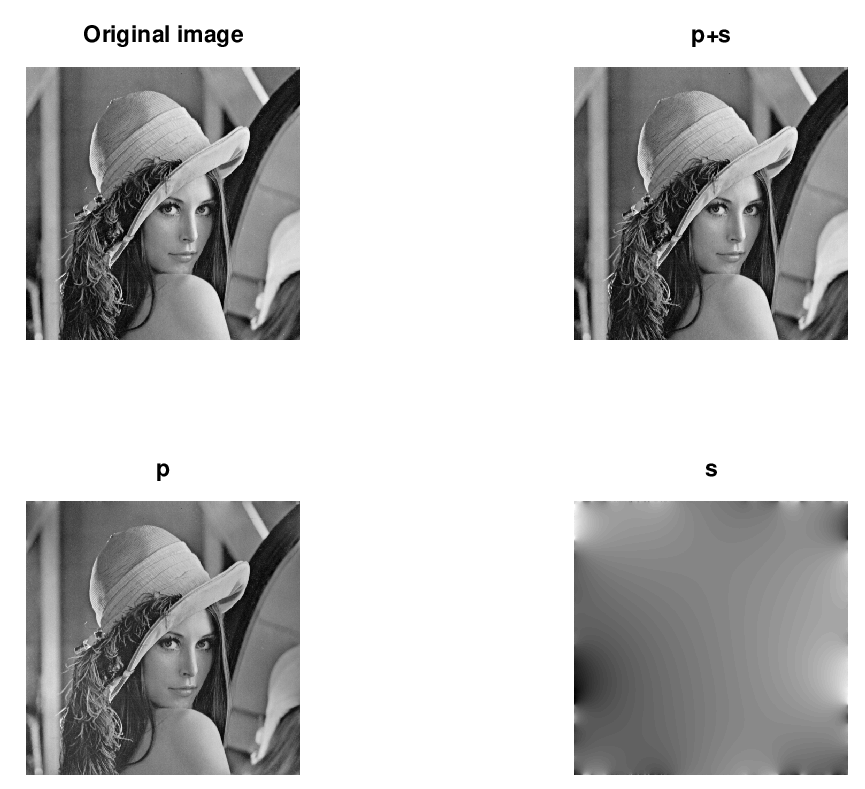
\includegraphics[width=12cm]{lena_perdecomp.png}
\caption{Décomposition $p+s$ de l'image “lena.pgm”}
\label{fig:decomp}
\end{figure}

Voici le code ayant produit l'image ci-dessus

\begin{lstlisting}[frame=single]
u = double(imread("lena.pgm"));
[p,s] = perdecomp(u);

subplot(2,2,1), imshow(u, [])
title("Original image")
subplot(2,2,2), imshow(p+s, [])
title("p+s")
subplot(2,2,3), imshow(p, [])
title("p")
subplot(2,2,4), imshow(s, [])
title("s")
\end{lstlisting}

On ajoute \texttt{[]} dans le \texttt{imshow} afin que la fonction \texttt{imshow} ajuste automatiquement les niveaux de noir et blanc
par rapport au minimum et au maximum de l'image qu'on lui donne en entrée. Comme attendu, l'image reconstruite par
\texttt{s+u} et l'image originale sont identiques: ce sont les deux images de la première ligne de la
figure~\ref{fig:decomp}.\\

Par rapport à l'image originale, l'image périodisée \texttt{p} est moins contrastée (cela se voit bien sur les cheveux de
Lena) et les niveaux de gris d'un bord à l'autre sont les mêmes horizontalement et verticalement. C'est précisément le
but de la periodisée: on veut effacer les discontinuités au bord du domaine qui apparaissent lors de la périodisation
forcée de l'image. On peut vérifier cela en simulant la périodisation de l'image et de sa décomposition \texttt{p+s}:
voir figure~\ref{fig:tile}.

\begin{figure}[!h]
\centering
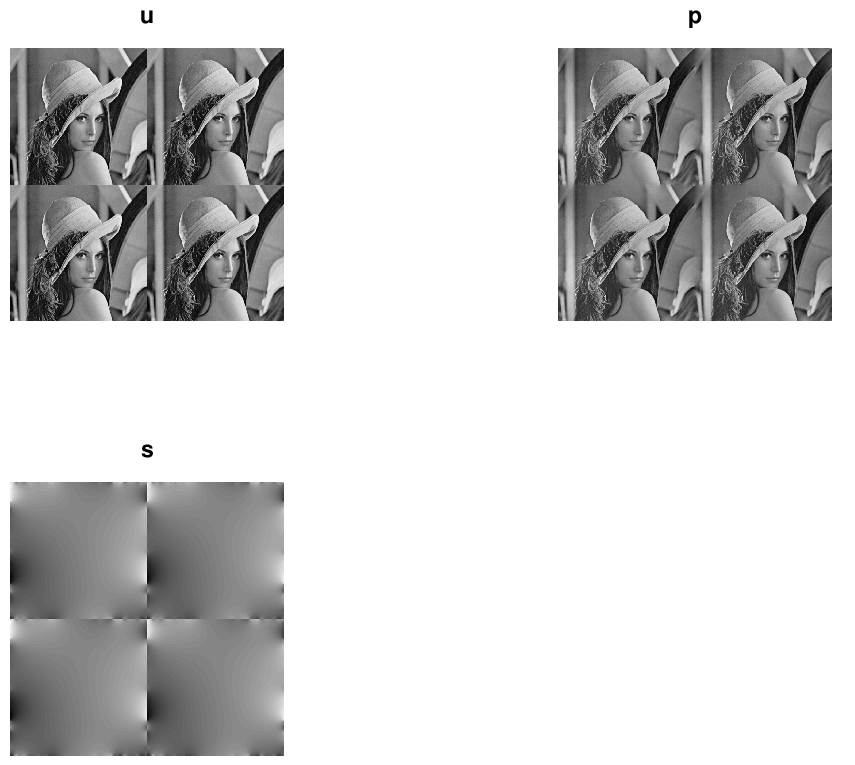
\includegraphics[width=14cm]{lena_perdecomp_tile.png}
\caption{Décomposition $p+s$ de l'image “lena.pgm” et simulation périodisation}
\label{fig:tile}
\end{figure}

On observe clairement la présence de discontinuités lors de la périodisation dans le plan de l'image originale alors que
ces discontinuités ont disparu pour la composante \texttt{p}. \\

Visualisons les effets de la décomposition $p+s$ sur le module et la phase de la transformée de Fourier.

\begin{figure}[!h]
\centering
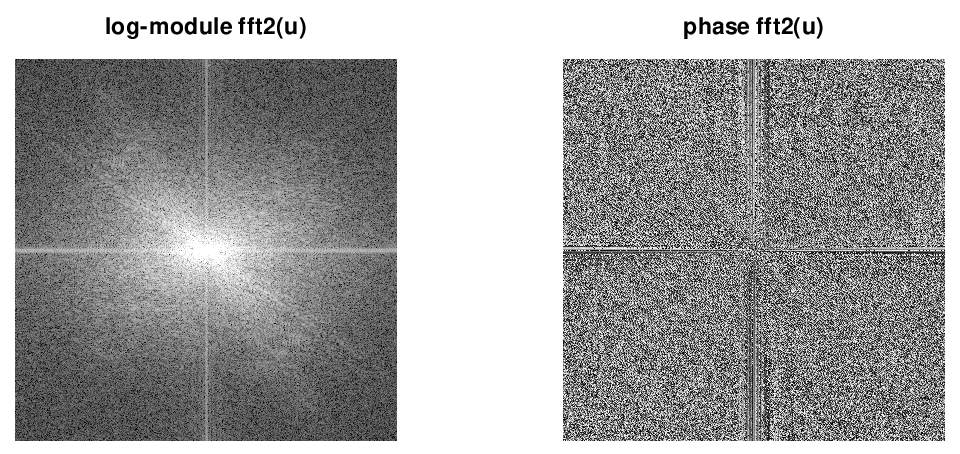
\includegraphics[width=10cm]{lena_fft_u.png}
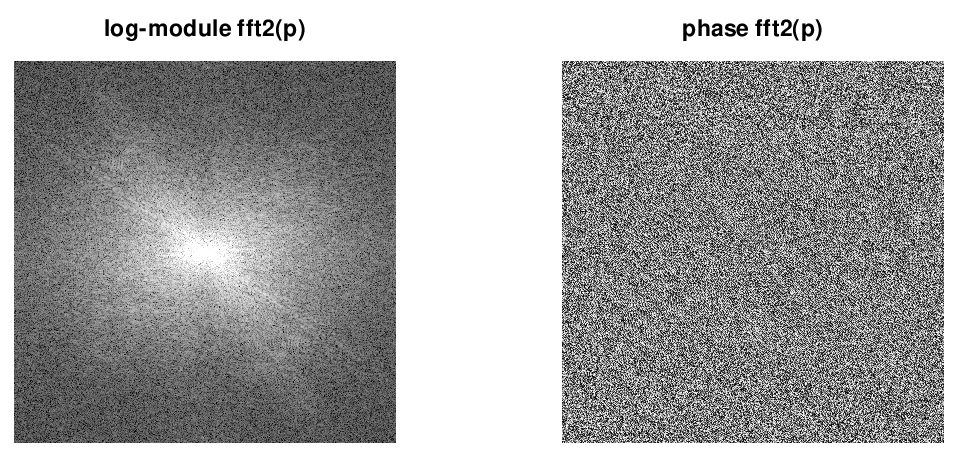
\includegraphics[width=10cm]{lena_fft_p.png}
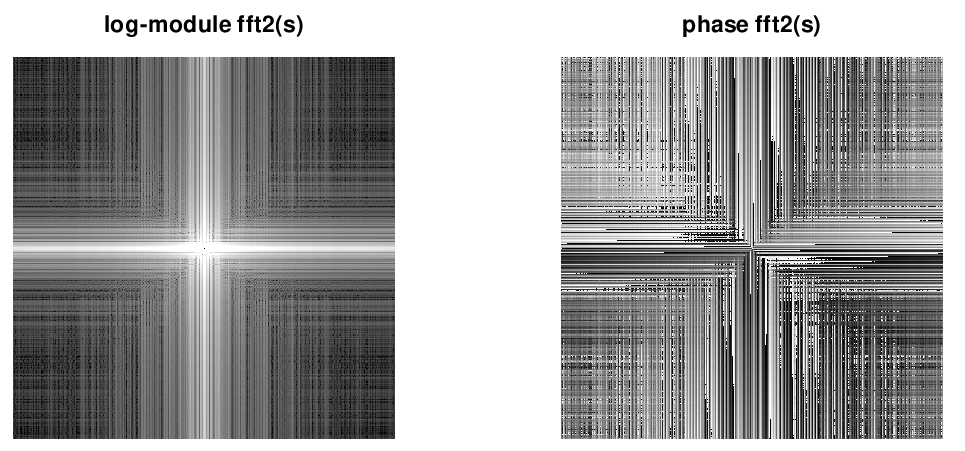
\includegraphics[width=10cm]{lena_fft_s.png}
\caption{Log-module et phase de la décomposition $p+s$ de l'image “lena.pgm”}
\label{fig:fft}
\end{figure}

Le code correspondant est

\begin{lstlisting}[frame=single]
fu = fft2(u);
fp = fft2(p);
fs = fft2(s);

subplot(1,2,1), imshow(normsat(fftshift(log(abs(fu))), 1));
title("log-module fft2(u)")
subplot(1,2,2), imshow(normsat(fftshift(angle(fu)), 1));
title("phase fft2(u)")
subplot(1,2,1), imshow(normsat(fftshift(log(abs(fp))), 1));
title("log-module fft2(p)")
subplot(1,2,2), imshow(normsat(fftshift(angle(fp)), 1));
title("phase fft2(p)")
subplot(1,2,1), imshow(normsat(fftshift(log(abs(fs))), 1));
title("log-module fft2(s)")
subplot(1,2,2), imshow(normsat(fftshift(angle(fs)), 1));
title("phase fft2(s)")
\end{lstlisting}

On observe nettement la différence entre l'image \texttt{u} et sa périodisée \texttt{p} dans le domaine de Fourier. La croix \og
parasite \fg qui apparait dans le module et la phase de la transformée de Fourier du \texttt{u} a disparu dans celle
de \texttt{p}. C'est justement l'effet de l'opérateur $per$: on fait disparaitre les discontinuités au bord du domaine
de l'image, lesquelles sont responsables sinon de grandes fréquences dans le domaine de Fourier le long des axes $x$ et
$y$ lors de la périodisation forcée de l'image. \\

Au lieu d'effectuer cette décomposition \texttt{s+p}, on peut forcer la continuité aux bords du domaine de l'image lors
de la périodisation spatiale en symétrisant l'image dans les deux directions. C'est la figure~\ref{fig:fsym}.

\begin{figure}[!h]
  \centering
  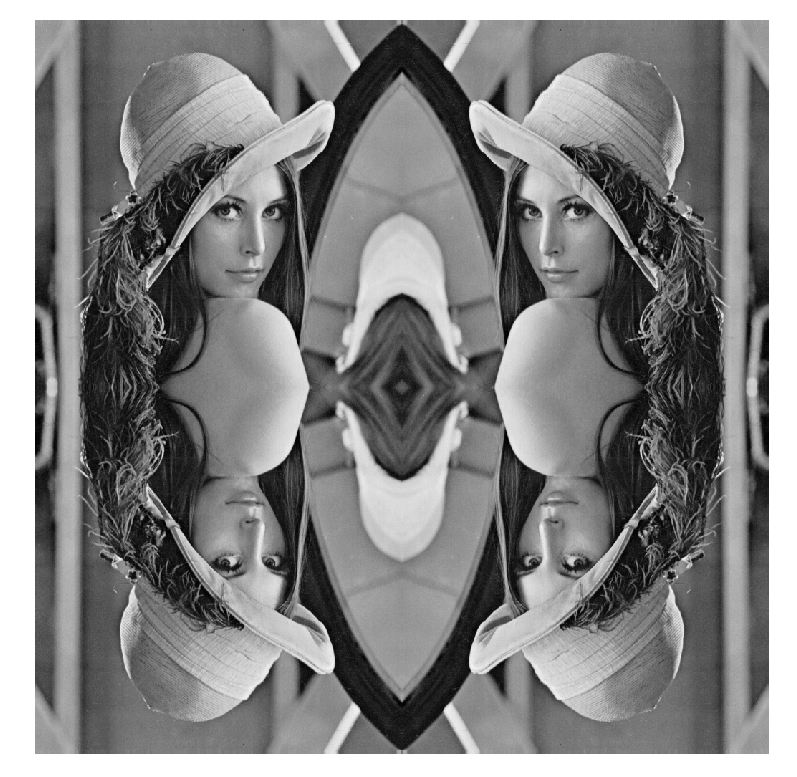
\includegraphics[width=6cm]{lena_fsym2.png}
  \caption{Symétrisée de “lena.pgm”}
  \label{fig:fsym}
\end{figure}

On prend alors le log-module et la phase de la transformée de Fourier de cette symétrisée pour obtenir la
figure~\ref{fig:ffsym}

\begin{figure}[!h]
  \centering
  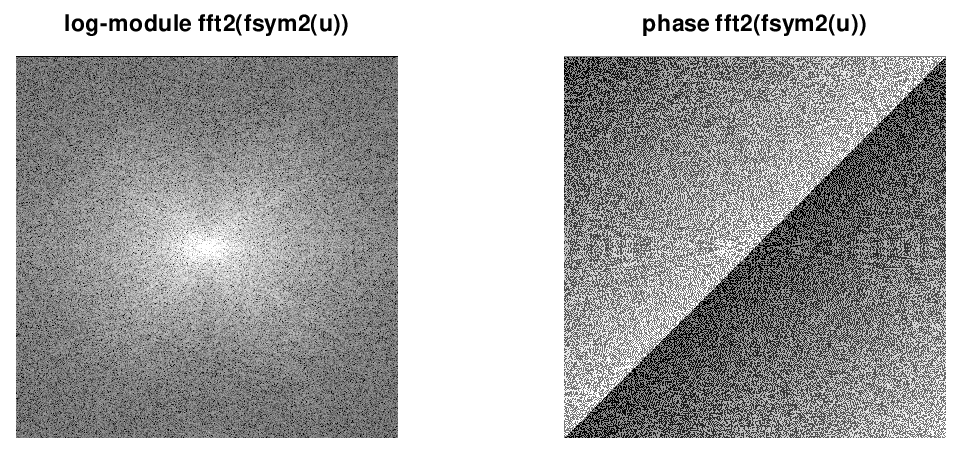
\includegraphics[width=14cm]{lena_fft_fsym2u.png}
  \caption{log-module et phase transformée de Fourier de la symétrisée de “lena.pgm”}
  \label{fig:ffsym}
\end{figure}

Tout comme la décomposition par l'opérateur $per$, la symétrisation lisse l'image aux bords de son domaine tel que la
périodisation forcée ne fait pas apparaître de discontinuité des valeurs. Néanmoins la symétrisation a le désavantage
par rapport à l'opérateur de $per$ d'introduire une discontinuité dans les valeurs des dérivées aux bords du domaine de
l'image.

\clearpage

\paragraph{Exercice 12}

Soit une image numérique $u: \Omega \to \mathbf{R}$ et $s$ l'application \og smooth \fg i.e $s=u - per(u)$. D'après le cours,
chacune des 4 propriétés suivantes caractérise $s$. 

\begin{enumerate}
  \item $s$ minimise $\displaystyle F(s) = \sum_{x \in \Omega, Y \in W(x)} \left( (u-s)(x) - (u-s)(y) \right)^2$ +
  $\displaystyle \sum_{x \in \Omega, Y \in V(x)} \left( s(x) - s(y) \right)^2$  + $\displaystyle \sum_{x \in \Omega} s(x)^2$
  \item $s = (Q_1 + Q_2)^{-1}Q_1u$ avec $Q_1 \succeq 0$,  $Q_2 \succ 0$
  \item $\Delta s = \Delta_{ext}u$ et $\displaystyle \sum_{x \in \Omega} s(x) = 0$
  \item $\hat{s}[0, 0] = 0$, $\hat{s}[q, r] = \frac{\hat{v}[q, r]}{\hat{k}[q, r]}$
\end{enumerate}

\textbf{1.} Montrer que $s$ ne dépend que de $u$ sur $\partial \Omega$ revient à montrer que $s$ ne dépend pas de $u(x)$
pour $x \in \mathring{\Omega}$. Soit un tel x. La caractérisation 3. nous donne alors le résultat. En effet $\Delta_{ext} 
u(x) = \sum_{y \in W(x)} u(x)-u(y)$ mais $W(x) = \emptyset$ mais pour le $x$ choisi. Ainsi peut importe la valeur de
$u(x)$, elle n'affecte pas l'équation qui caractérise $s$. C'est donc que $s$ est indépendant de cette coordonnée. \\

\textbf{2.} A nouveau on utilise la caractérisation 3. Soit $x \in \mathring{\Omega}$, alors $W(x) = \emptyset$. La
somme sur un ensemble vide est par convention nulle, d'où $\Delta s(x) = 0$. s est harmonique sur $\mathring{\Omega}$.\\

\textbf{3.} Montrons tout d'abord que l'application $per : \mathbf{R}^{\Omega} \to \mathbf{R}^{\Omega}$ est linéaire.
Soient $u, v \in \mathbf{R}^{\Omega}$, $\lambda \in \mathbf{R}$. On note

\begin{align*}
  s_{u+\lambda v} &= u + \lambda v - per(u+\lambda v) \\
  s_u &= u - per(u) \\
  s_v &= v - per(v)
\end{align*}

Par linéarité du Laplacien et de $\Delta_{ext}$ (évident) 

\begin{align*}
  \Delta (s_u + \lambda s_v) &= \Delta s_u + \lambda \Delta s_v \\
  &= \Delta_{ext}u + \lambda \Delta_{ext}v \\
  &= \Delta_{ext}(u+\lambda v) 
\end{align*}

Par ailleurs $\displaystyle \sum_{x \in \Omega} (s_u + \lambda s_v) (x) = 0 + \lambda 0 = 0$. Comme la condition 3.
caractérise $s_u$ pour $u$ donné, on a $s_{u+\lambda v} = s_u + \lambda s_v$ d'où $per(u + \lambda v) = per(u) +
\lambda per(v)$.  \\

$per$ est un endomorphisme de l'espace vectoriel de dimension finie $\mathbf{R}^{\Omega}$. Alors $per$ est bijective si
elle seulement si son noyau est réduit à 0. Soit $u$ tel que $per(u)=0$. En utilisant la caractérisation 2. on a alors
$u = (Q_1 + Q_2)^{-1}Q_1u$ i.e $(Q_1 + Q_2)u = Q_1u$ d'où $Q_2u = 0$. Mais $Q_2$ est définie positive d'où $u=0$. \\

\textbf{4.} Soit $(v, \lambda)$ un vecteur propre de $per$ et sa valeur propre associée. Alors $v - per(v) =
(1-\lambda)v$ d'où en utilisant la caractérisation 3. $(Q_1 + Q_2)(1-\lambda)v = Q_1 v$. Cetter dernière équation
est équivalente à $(1-\lambda)Q_2 v = \lambda Q_1 v$. \\

Supposons $\lambda \neq 1$. Alors $Q_2 v = \frac{\lambda}{1-\lambda}Q_1v$. Comme $Q_1 \succeq 0$,  $Q_2 \succ 0$, on a
$v^T Q_2 v > 0$ et $v^T Q_1 v >= 0$. On en déduit 

\begin{equation*}
  \frac{\lambda}{1-\lambda} > 0
\end{equation*}

Cette équation signifie deux choses: le quantité $\frac{\lambda}{1-\lambda}$ est réelle et strictement positive. En
écrivant $\lambda$ sous forme algébrique $a+ib$ on montre que $\frac{\lambda}{1-\lambda} \in \mathbf{R} \implies b=0$ i.e
$\lambda$ réel. Ensuite une simple étude de signe montre que $\lambda \in ]0,1[$. En résumé soit $\lambda = 1$ soit
$\lambda$ est réel et dans $]0,1[$ c'est-à-dire $\lambda$ réel et dans $]0,1]$. \\

\textbf{5.} Soit $u$ un point fixe de $per$ i.e $per(u) = u$. D'après 3. on a alors $Q_1u=0$ et donc a fortiori
$u^TQ_1u=0$. Mais on a aussi

\begin{equation*}
u^TQ_1u = \sum_{x \in \Omega, Y \in W(x)} \left( u(x) - u(y) \right)^2
\end{equation*}

Cette somme est nulle si et seulement si tous ces termes sont nuls. Ainsi $\forall x \in \Omega, \forall y \in W(x),
u(y)=u(x)$. \\

Réciproquement supposons que $u$ soit tel que $\forall x \in \Omega, \forall y \in W(x), u(y)=u(x)$. Alors $s=0$ est
un minimiseur évident de $F$. Étant donné que 1. caractérise $s$, on a bien $s=0$ i.e $per(u)=u$. \\

\textbf{6.} D'après le théorème donné en indication, il existe $P$ inversible et $D$ diagonale telles que

\begin{align*}
  P^TQ_1P &= D \\
  P^TQ_2P &= I
\end{align*}

La matrice représentant $per$ dans la base canonique de $\mathbf{R}^{\Omega}$ est $I-(Q_1+Q_2)^{-1}Q_1$ d'après 3. Or
$P^T(Q_1+Q_2)P = D+I$ d'où $(Q_1+Q_2)^{-1} = P(D+I)^{-1}P^T$. Comme $Q_1 = P^{-T}DP^{-1}$ on a

\begin{align*}
  I-(Q_1+Q_2)^{-1}Q_1 &= I - P(D+I)^{-1}P^T P^{-T}DP^{-1}\\
    &= P(I - (D+I)^{-1}D)P^{-1}
\end{align*}

La matrice centrale est diagonale.  $I-(Q_1+Q_2)^{-1}Q_1$  est donc diagonalisable d'où $per$ est diagonalisable.\\

\end{document}

